\documentclass[french, a4paper, 12pt, titlepage]{article}
%% Peut remplacer "article" par "scrartcl" %%

\usepackage{a4wide}
%\usepackage[top=2cm, bottom=2cm, left=2cm, right=2cm]{geometry}
\raggedbottom % prevents vertical white space on pages that cannot be filled properly

\usepackage{hyperref}
\hypersetup{
	colorlinks=true,       	% false: boxed links; true: colored links
	linkcolor=black,          	% color of internal links
	urlcolor=blue,           	% color of external links
	citecolor=grey
}

\usepackage[T1]{fontenc}
%\usepackage{fourier}
%\usepackage{utopia}
%\usepackage{palatino}

\usepackage{lmodern}
%% ajouter fonte petite capitale grasse à lmodern avec celle de computer modern %%
\rmfamily
\DeclareFontShape{T1}{lmr}{b}{sc}{<->ssub*cmr/bx/sc}{}
\DeclareFontShape{T1}{lmr}{bx}{sc}{<->ssub*cmr/bx/sc}{}
%% /ajout %%
\usepackage{wrapfig}

%\usepackage[a4paper]{geometry} % marges plus petites que a4paper standard
\usepackage{listings} % insérer code source
%\usepackage{algorithm} % algorithmique
%\usepackage{algorithmic}
\usepackage{url}
\usepackage[usenames, dvipsnames]{color} % couleurs (nombre de base étendu)
\usepackage{graphicx} % insérer images
\usepackage[utf8]{inputenc}
\usepackage[french]{babel}
\usepackage{amsmath}
\usepackage{amsfonts}
\usepackage{amssymb}
\usepackage{amsthm}
\usepackage{multicol}
\definecolor{grey}{rgb}{0.96,0.96,0.96}
\definecolor{grey2}{rgb}{0.3,0.3,0.3}

%% Define listings params %%
\lstset{
	numbers=left,
	language=Java,
	tabsize=4,
	frame=single, % cadre autour du code
	breaklines=true, % autorise couper ligne trop longue
	basicstyle=\small\ttfamily,
	numberstyle=\scriptsize\ttfamily,
	backgroundcolor=\color{grey},
	showstringspaces=false,
	keywordstyle=\color{OliveGreen},
	stringstyle=\color{BrickRed},
	commentstyle=\color{grey2}\it,
	stepnumber=1
} % numérote toute les x lignes
% listing utf8 fr %
\lstset{%
	inputencoding=utf8,
	extendedchars=true,
	literate=
		{é}{{\'{e}}}1
		{è}{{\`{e}}}1
		{ê}{{\^{e}}}1
		{ë}{{\¨{e}}}1
		{û}{{\^{u}}}1
		{ù}{{\`{u}}}1
		{â}{{\^{a}}}1
		{à}{{\`{a}}}1
		{î}{{\^{i}}}1
		{ç}{{\c{c}}}1
		{Ç}{{\c{C}}}1
		{É}{{\'{E}}}1
		{Ê}{{\^{E}}}1
		{À}{{\`{A}}}1
		{Â}{{\^{A}}}1
		{Î}{{\^{I}}}1
}
%% /Define listings params %%

%% Francisation des algorithmes
%\renewcommand{\algorithmicrequire} {\textbf{\textsc{Entrées:}}}
%\renewcommand{\algorithmicensure}  {\textbf{\textsc{Sorties:}}}
%\renewcommand{\algorithmicwhile}   {\textbf{tant que}}
%\renewcommand{\algorithmicdo}      {\textbf{faire}}
%\renewcommand{\algorithmicendwhile}{\textbf{fin tant que}}
%\renewcommand{\algorithmicend}     {\textbf{fin}}
%\renewcommand{\algorithmicif}      {\textbf{si}}
%\renewcommand{\algorithmicendif}   {\textbf{fin si}}
%\renewcommand{\algorithmicelse}    {\textbf{sinon}}
%\renewcommand{\algorithmicthen}    {\textbf{alors}}
%\renewcommand{\algorithmicfor}     {\textbf{pour}}
%\renewcommand{\algorithmicforall}  {\textbf{pour tout}}
%\renewcommand{\algorithmicdo}      {\textbf{faire}}
%\renewcommand{\algorithmicendfor}  {\textbf{fin pour}}
%\renewcommand{\algorithmicloop}    {\textbf{boucler}}
%\renewcommand{\algorithmicendloop} {\textbf{fin boucle}}
%\renewcommand{\algorithmicrepeat}  {\textbf{répéter}}
%\renewcommand{\algorithmicuntil}   {\textbf{jusqu'à}}
%\renewcommand{\algorithmiccomment} {\STATE //}
%\newcommand{\BEGIN}{\STATE \fbox{Début}}
%\newcommand{\END}{\STATE \fbox{Fin}}
%\floatname{algorithm}{Algorithme}
%% /francisation des algorithmes

\renewcommand{\qedsymbol}{}

\newcommand{\petit}[1]{
	\medskip \noindent
	\begin{small}
	#1)
	\end{small}
}

\begin{document}

\title{Atelier Systèmes d'Exploitation}
\author{\textsc{Martel} Damien}
\date{Compilé le \today}

\maketitle
%% Laisse page blanche pour verso page de garde %%

\vfill
\pagebreak

%\tableofcontents
\newpage
\strut\thispagestyle{empty}
\vfill
\pagebreak
\tableofcontents
\strut\thispagestyle{empty}
%\setcounter{page}{0}
\newpage
\setcounter{page}{1}

\section{Questions pré-projet}
\begin{enumerate}
\item \textbf{Combien de processus seront créés dans le projet ?}\\
Les différents acteurs du projet sont: \begin{itemize}
\item Les terminaux
\item Les serveurs d'acquisition
\item Les serveurs interbancaires
\item Les serveurs d'autorisation
\end{itemize}
Nous aurons donc un minimum de 4 processus.
Dans la réalité nous pouvons avoir plusieurs banques \textit{(N banques)} et plusieurs terminaux de paiement \textit{(M terminaux)}, nous pourrons avoir donc au maximum $1+2N+M$ processus.\\

\item \textbf{Combien d'exécutables allez-vous programmer ? Est ce que un seul exécutable est acceptable ?}\\
Parmi les 4 acteurs précédents 3 d'entres eux se retrouvent éloigné géographiquement, (le client, sa banque et le serveur interbancaire).
C'est 3 entités représentent 3 serveurs physique et faire moins d'exécutables que ça ne permettrais pas de passer de la simulation à la réalité.\\

\item \textbf{Qui (quel processus) est créé par qui ?}\\
Pour rester le plus fidèle à la réalité, chaque processus est lancé indépendemment.\\

\item \textbf{Dessinez l'arbre des processus du projet.}
\smallskip
\begin{center}
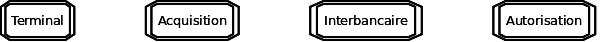
\includegraphics[scale=0.3]{fork}
\end{center}

\item \textbf{Combien de tubes sont nécessaires pour le projet ?}\\
Pour le projet, nous avons une paire de tube par terminaux, et deux paires par banque soit, $4N+2M$ tubes.\\

\item \textbf{Quels types de tubes allez-vous utiliser ?}
Les tubes nommées (fifo) paraissent le plus approprié, pour faire communiquer deux processus qui n'ont pas de liens de parenté.\\

\item \textbf{Qui (quel processus) crée quels tubes ?}\\
Les terminaux créent les $2M$ tubes les reliant à leurs banque respectif, et les banques les $2N$ tubes les reliants aux serveur interbancaire.\\

\item \textbf{Dessinez vos processus et vos tubes.}\\

\end{enumerate}

\end{document}
